\chapter{Сэдвийн ерөнхий судалгаа}

Сэдвийн хүрээнд өмнө нь ажиллаж үзээгүй олон шинэ технологиудыг судалж хэд хэдэн шинэ технологи ашиглаж, тэдгээрийг үнэлж, харьцуулав. Энэ бүлэгт би судалгаанаасаа сонгосон технологиудыг танилцуулж, вэб платформыг бий болгох үндсэн ойлголтуудыг танилцуулж байна.

\section{Үндсэн ойлголтууд}

Энэхүү судалгааг амжилттай дуусгахын тулд зарим үндсэн ойлголтуудыг ойлгох нь зайлшгүй чухал юм.

\subsection{Web Sockets}

WebSocket нь хэрэглэгчийн хөтөч болон серверийн хооронд хоёр талын интерактив харилцааны session нээх боломжтой дэвшилтэт технологи юм. Энэхүү WebSocket - ийн тусламжтайгаар сервер рүү мэдээлэл илгээж, серверээс хариулт авах шаардлагагүйгээр үйл явдалд тулгуурласан хариултуудыг хүлээн авах боломжтой.

\begin{itemize}

	\item Real-time Interaction: Хэрэглэгчдийг бодит цаг хугацаанд бие биетэйгээ уралдуулахыг хүсвэл WebSockets маш чухал. Тэд оролцогч бүрийн мэдээллийг бусад бүх оролцогчдын дэлгэцэн дээр нэн даруй шинэчлэх боломжийг олгоно.
	\item Dynamic Updates: Хэрэв тоглоомын орчин, дүрэм, зард ямар нэгэн өөрчлөлт орсон бол WebSockets нь бүх идэвхтэй хэрэглэгчдэд шууд мэдэгдэх боломжтой
	\item Multiplayer Racing: Олон оролцогчтой уралдааны хувьд тоглоомын төлөвийг удирдаж, хэрэглэгчдэд синхрончлолыг хангах нь WebSockets-ийн тусламжтай илүү удирдах боломжтой болно.
\end{itemize}

WebSockets нь бодит цагийн интерактив платформын салшгүй технологийн нэг бөгөөд шуурхай шинэчлэлт, харилцан үйлчлэлд шаардагдах хурд, үр ашгийг санал болгодогоороо давуу талтай.

\subsection{Web-based Educational Platforms}

Вэб дээр суурилсан платформууд нь хэрэглэгчид хүссэн үедээ, хаанаас ч, ихэвчлэн өөрийн хүссэн хэмжээгээр систем руу хандах боломжтойгоороо давуу талтай.

Өрсөлдөх чадвартай эсвэл хамтран ажиллах боломжуудыг агуулж, суралцахыг нийгмийн туршлагыг бий болгож хэрэглэгчид дэлхийн хэмжээнд үе тэнгийнхэнтэйгээ өрсөлдөх эсвэл тэднээс суралцах боломжтой.
\section{Ижил төсөөтэй систем}

\subsection{TypingTest.com}

"TypingTest Pro" нь хэрэглэгчид бичих хурд, нарийвчлалыг хэмжихэд зориулагдсан онлайн платформ юм. Энэ платформ нь хэрэглэгчдэд бодит цагийн горимд бичих янз бүрийн текстүүдийг өгч, гүйцэтгэлийн талаар шууд санал хүсэлтийг санал болгодог.

\begin{figure}[h]
	\centering
	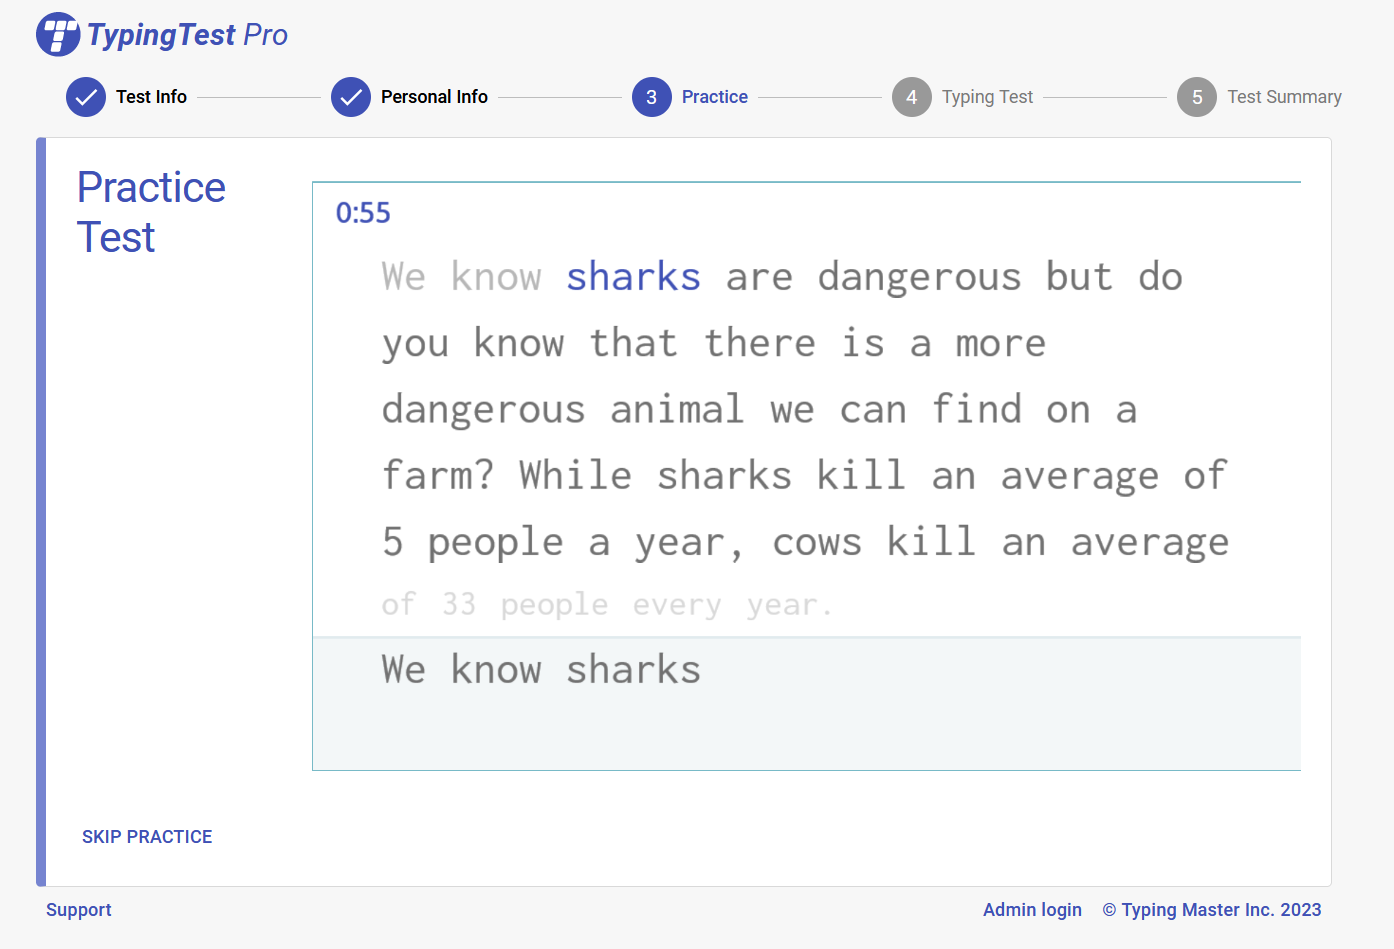
\includegraphics[width=15cm]{images/typingtestpro.png}
	\caption{typingtest.com/pro/ сайтын харагдах байдал}
	\label{fig:alltop}
\end{figure}

Манай бүтээх гэж байгаа вебээс ялгаатай тал нь
\begin{itemize}
	\item 1-ээс 10 минутын хугацаатай туршилтуудыг санал болгож, хэрэглэгчдэд сорилтын түвшингээ сонгох боломжийг олгодог.
	\item Шууд guest хэлбэрээр орон тест өгөх боломжгүй
\end{itemize}

Frontend: HTML5, CSS3 болон динамик хэрэглэгчийн интерфэйсүүдэд зориулсан React.js-тэй JavaScript.
Backend: Express.js хүрээтэй Node.js нь өргөтгөх боломжтой, үр ашигтай сервер талын програмыг хангадаг.
Өгөгдлийн сан: Хэрэглэгчийн профайл, тестийн үр дүн, текстийн хэсгүүдийг хадгалах MongoDB.WebSockets: Бодит цагийн өрсөлдөөн, шууд санал хүсэлтийн функцэд зориулагдсан.
Third-party Integrations: Дэлхий даяар тэргүүлэгчдийн самбар, олон нийтийн мэдээллийн хэрэгслээр хуваалцах боломжууд.

Онлайнаар шивэх тестийн олон платформууд байдаг ч "TypingTest Pro" нь энгийн хэрэглэгчид болон бичих чадвараа сайжруулахад нухацтай ханддаг хүмүүст зориулсан иж бүрэн функцээрээ бусдаас ялгардаг.

\subsection{play.typeracer.com}

TypeRacer бол олон тоглогчийн онлайн хөтөч дээр суурилсан шивэх тоглоом юм. Тоглогчид богино хэсгийг аль болох хурдан шивэх замаар өрсөлддөг бөгөөд тоглоом нь хурдыг минут тутамд үгээр (WPM) болон нарийвчлалыг хэмждэг. Үүсгэн байгуулагдсан цагаасаа эхлэн энэ нь өрсөлдөөнтэй, хөгжилтэй орчинд бичих чадвараа сайжруулахыг хүсч буй хүмүүсийн дуртай хэрэгсэл болсон.

\begin{figure}[h]
	\centering
	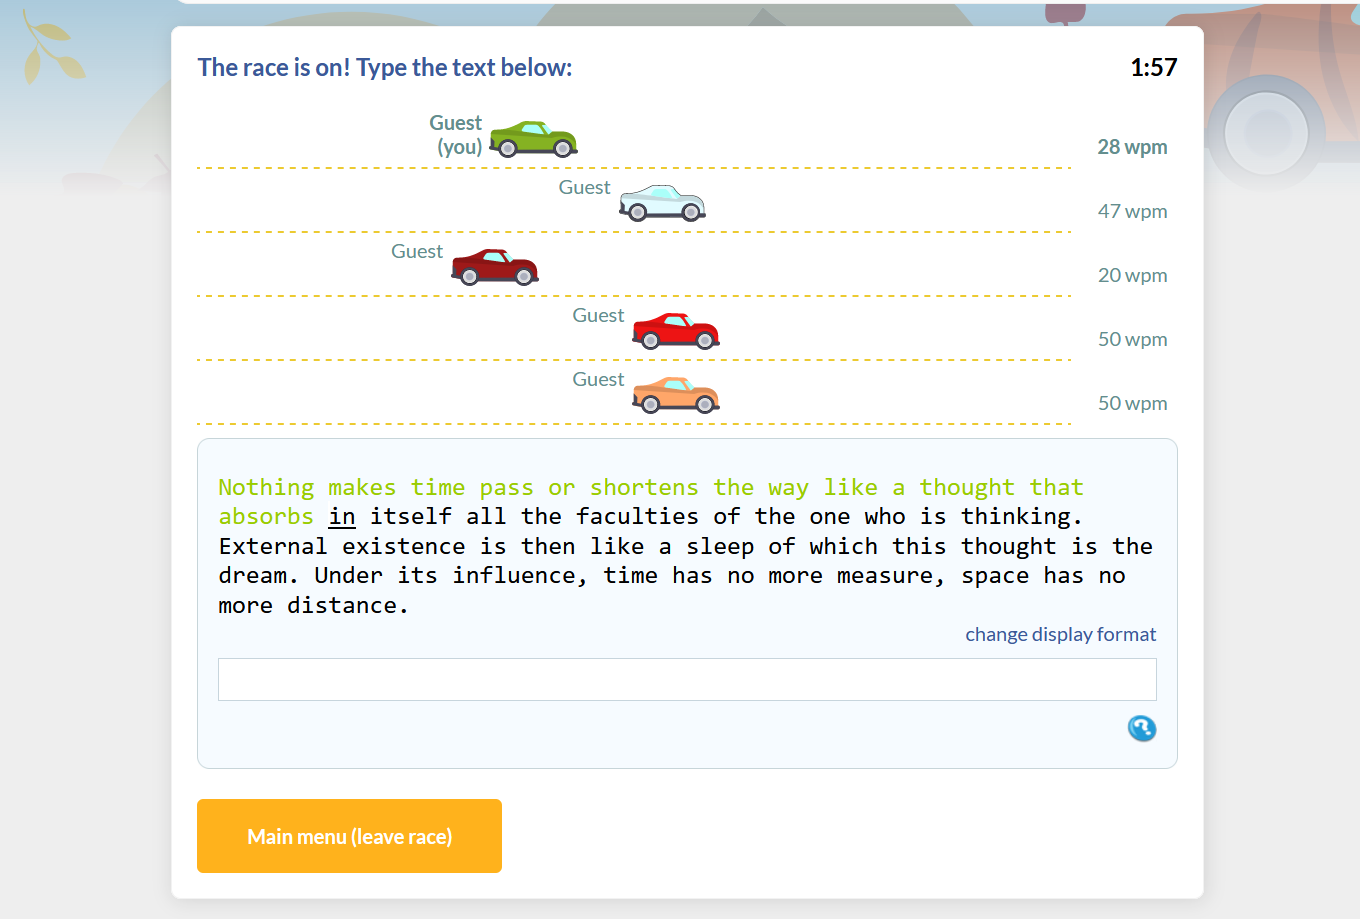
\includegraphics[width=15cm]{images/TypeRacer.png}
	\caption{play.typeracer.com сайтын харагдах байдал}
	\label{fig:linktree}
\end{figure}

Гол онцлог:

Энэ бол вэб дээрх анхны олон тоглогчийн шивэх тоглоом юм.

2008 оны 3-р сард нээлтээ хийснээс хойш дэлхийн өнцөг булан бүрээс сая сая хүмүүс typeracer.com сайт дээр хэдэн зуун сая уралдаанд оролцож, бичих хурдаа минут тутамд 50 үгээр сайжруулсан.

TypeRacer нь 50 өөр хэл дээр байдаг.

2010 онд гарсан TypeRacer School Edition нь дэлхийн хамгийн хөгжилтэй боловсролын бүтээгдэхүүн болох зорилготой юм. K-12 сургуулиудад зориулагдсан бөгөөд бичихийг спорт болгон хувиргаж, суралцахыг хөгжилтэй болгодог TypeRacer тоглоомын үзэл баримтлалыг ашигладаг.
\section{Ашиглах технологи}

\subsection{Figma - интерфейс дизайн, Prototype хувилбар гаргах багаж}
Figma нь хэрэглэгчдэд нэг платформ дээр дизайн хийх, загвар гаргах, санал хүсэлтийг цуглуулах боломжийг олгодог дизайны хэрэгсэл юм. Дизайнерууд, хөгжүүлэгчид, бүтээгдэхүүний менежерүүд болон оролцогч талууд бодит цаг хугацаанд хамтран ажиллах боломжтой бөгөөд энэ нь дижитал бүтээгдэхүүн дээр ажилладаг багуудад хүчирхэг хэрэгсэл болгодог.

Figma ашиглахын давуу талууд
\begin{itemize}
	\item Вэб дээр суурилсан бөгөөд энэ нь том хэмжээний програм хангамжийн багц татаж авах шаардлагагүй. Windows, MacOS, Linux зэрэг өөр өөр үйлдлийн системүүд дээр саадгүй ажилладаг
	\item Хийсэн өөрчлөлтүүдийг автоматаар хадгалж, шаардлагатай бол хуучин өөрчлөлт рүү буцах боломжийг олгодог
	\item Figma нь оюутнуудад нэмэлт зардал гаргахгүйгээр иж бүрэн төсөл хэрэгжүүлэх боломжийг үнэ төлбөргүй санал болгодог.
\end{itemize}

\begin{figure}[h]
	\centering
	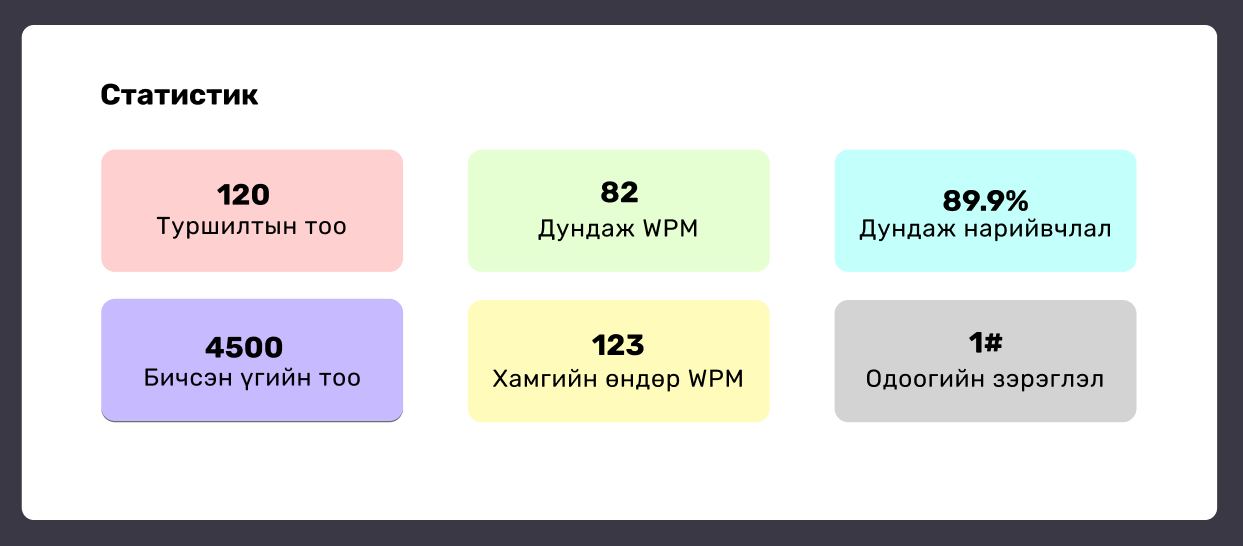
\includegraphics[width=10cm]{images/figma_component.png}
	\caption{Figma ашиглаж хийсэн компонент}
	\label{fig:figma}
\end{figure}

Зурсан интерфейсүүдээ хооронд нь холбож хийсвэрээр аппаа ажиллуулан хэрэглэгчийн туршилт хийх хэсгийг Prototype гэдэг бөгөөд заавал кодын хэрэгжүүлэлт хийж цаг хугацаа болон мөнгөн зардал гаргалгүйгээр хийж буй аппаа хэрэглэгчээр туршуулах, үр дүнгээ гарган авч түүнийгээ сайжруулах нөхцөлийг уг веб аппликейшн маань гаргаж өгсөн нь UX/UI дизайнеруудын ашиглах болсон хамгийн том шалтгаануудын нэг юм.

\subsection{Next.js - React дээр суурилсан фрэймворк}

\subsubsection{Сонгосон шалтгаан}

Энгийнээр хэлэхэд Next.js нь Javascript програмуудыг хөгжүүлэхэд зориулагдсан React framework юм. Вэб платформыг өндөр гүйцэтгэлтэй, өргөтгөх боломжтой, зөвхөн код дээрээ анхаарал хандуулах боломжийг олгож хурдан ажилладаг.

Next.js давуу талуудаас дурьдвал:
\begin{itemize}
	\item Вэб програмуудыг бүтээхэд хялбар бүтэцтэй
	\item Automatic code splitting JS болон CSS шаардлагагүй бол заавал татаж авдаггүй 
	\item Zero config буюу нэг ч тохиргоо хийлгүйгээр төслөө эхлүүлэх боломж
	\item Server Side Render хийх (SSR)
	\item Typescript болон Fast Refresh дэмждэг
	\item HRM болон хөгжүүлэгчдэд ээлтэй хэрэгслүүдтэй
	\item API Routes буюу өөр дээрээ nodejs сервер ашиглаж API endpoint гаргах боломжтой. Ингэснээр тусдаа сервер ашиглах шаардлага үүсэхгүй
	\item SEO буюу хайлтын системийн оновчлолыг SSR ашиглаж тохируулж өгөх
\end{itemize}

Хөгжүүлэлтийг хялбарчлаж хөгжүүлэгчдэд ээлтэй орчинг бүрдүүлэх чадвартай тул Next.js-ийг сонгов.

\subsubsection{Технологийн талаар}

Next.js\footnote{Next.js official site \url{https://nextjs.org}} нь уян хатан React дээр суурилсан фрэймворк бөгөөд хурдан вэб програмуудыг чанартай үүсгэх боломжийг өгдөг билээ. 


\subsection{Firebase - Өгөгдлийн сан}

Firebase бол Google-ээс гаргасан гар утас болон вэб програм хөгжүүлэх цогц платформ юм. Энэ нь хөгжүүлэгчдэд програмуудыг хурдан бөгөөд үр дүнтэй бүтээх, сайжруулах, масштаблахад туслах өргөн хүрээний хэрэгсэл, үйлчилгээг санал болгодог. Firebase нь янз бүрийн функц, үйлчилгээг багтаасан бөгөөд үүнийг програм хөгжүүлэхэд түгээмэл сонголт болгодог. Firebase-ийн зарим үндсэн бүрэлдэхүүн хэсэг, боломжуудыг энд харуулав.


Firebase давуу талуудаас дурьдвал:
\begin{enumerate}
	\item Real-time Database энэ функц нь холбогдсон бүх үйлчлүүлэгчид тоглоомын өгөгдлийг шуурхай шинэчлэх боломжийг олгож, олон тоглогчийн туршлагыг тасралтгүй бий болгодог.
	\item Authentication бүртгэл, нэвтрэх функцийг хэрэгжүүлэхэд хялбар болгодог
	\item Serverless Functions эдгээр функцийг тоглоомын session удирдлага, онооны тооцоо зэрэг сервер талын логикийг хэрэгжүүлэхэд ашиглаж болно.
	\item Cost efficiency боломжийн үнэ бүхий, төлбөргүй олон боломжуудыг санал болгодог
\end{enumerate}

\begin{figure}[h]
	\centering
	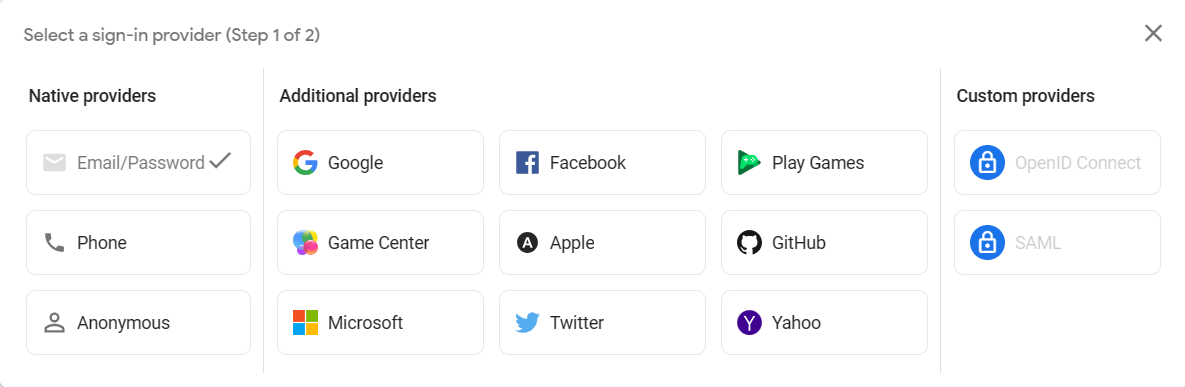
\includegraphics[width=15cm]{images/firebase_auth.png}
	\caption{Firebase Authentication}
	\label{fig:prisma}
\end{figure}

Firebase-ийг бодит цагийн харилцан үйлчлэл, authentication зэргийг төслийн гол бүрэлдэхүүн хэсэг болгон хэрэглэх болно.

\subsection{Socket.io - Library}

Socket.IO бол бодит цагийн вэб програмуудад зориулсан үйл явдалд суурилсан сан юм. Энэ нь вэб үйлчлүүлэгч болон серверүүдийн хооронд бодит цагийн, хоёр чиглэлтэй харилцаа холбоог идэвхжүүлдэг. Энэ нь үйлчлүүлэгч, сервер гэсэн хоёр бүрэлдэхүүн хэсгээс бүрдэнэ.